\documentclass[12pt]{article}
\usepackage[a4paper, left=3.17cm, right=3.17cm, top=2.54cm, bottom=2.54cm]{geometry}
\usepackage[fontset=mac]{ctex}
\usepackage[T1]{fontenc}
\usepackage{mathptmx}
\usepackage{amsfonts}
\usepackage{amsmath,amssymb,amsthm}
\usepackage{enumerate}
\usepackage{graphics}
\usepackage{chemformula}
\usepackage{cite}
\usepackage[colorlinks, linkcolor=black, anchorcolor=black, citecolor=black]{hyperref}
\usepackage{indentfirst}
\usepackage{listings}
\lstset{breaklines}
\lstset{ %
	extendedchars=false,            % Shutdown no-ASCII compatible
	language=C++,                % choose the language of the code
	basicstyle=\footnotesize\tt,    % the size of the fonts that are used for the code
	tabsize=3,                            % sets default tabsize to 3 spaces
	numbers=left,                   % where to put the line-numbers
	numberstyle=\tiny,              % the size of the fonts that are used for the line-numbers
	stepnumber=1,                   % the step between two line-numbers. If it's 1 each line
	% will be numbered
	numbersep=5pt,                  % how far the line-numbers are from the code   %
	keywordstyle=\color[rgb]{0,0,1},                % keywords
	commentstyle=\color[rgb]{0.133,0.545,0.133},    % comments
	stringstyle=\color[rgb]{0.627,0.126,0.941},      % strings
	backgroundcolor=\color{white}, % choose the background color. You must add \usepackage{color}
	showspaces=false,               % show spaces adding particular underscores
	showstringspaces=false,         % underline spaces within strings
	showtabs=false,                 % show tabs within strings adding particular underscores
	frame=single,                 % adds a frame around the code
	captionpos=b,                   % sets the caption-position to bottom
	breaklines=true,                % sets automatic line breaking
	breakatwhitespace=false,        % sets if automatic breaks should only happen at whitespace
	title=\lstname,                 % show the filename of files included with \lstinputlisting;
	% also try caption instead of title
	mathescape=true,escapechar=?    % escape to latex with ?..?
	escapeinside={\%*}{*)},         % if you want to add a comment within your code
	columns=fixed,                  % nice spacing
	%morestring=[m]',                % strings
	morekeywords={%,...},%          % if you want to add more keywords to the set
	   break,case,catch,continue,elseif,else,end,for,function,global,%
	   if,otherwise,persistent,return,switch,try,while,...},%
}
\usepackage{graphicx}
\setlength{\parskip}{0.5em}
\title{《高性能计算引论》第三次作业}
\author{\textup{罗文水}}
\begin{document}
	\begin{titlepage}
		\newcommand{\HRule}{\rule{\linewidth}{0.5mm}}
		\begin{center}
			
\includegraphics[width=8cm]{../HPC_P1/title}			
		\end{center}
		
		\center 
		\quad\\[1.5cm]
		\textsl{\Large \textbf{Nanjing University of Science and Technology} }\\[0.5cm] 
		\textsl{\large School of Computer Science and Engineering}\\[0.5cm] 
		\makeatletter
		\HRule \\[0.4cm]
		{ \huge \bfseries \@title}\\[0.25cm] 
		\HRule \\[1.5cm]
	\begin{minipage}{0.42\textwidth}
		\begin{flushleft}
			
			\Large{\emph{姓名:罗文水}}
			\\
			\Large{\emph{学号:918106840738}}
			\\
			\Large{\emph{班级:计科一班}}
			\\
			\Large{\emph{课程:高性能计算引论}}
			\\
			\Large{\emph{授课教师:李翔宇}}
			\\
		\end{flushleft}
	\end{minipage}
		\vspace{7em} 
		
		{\large \today}\\[2cm] 
		\vfill 
	\end{titlepage}
	
	\newpage
\section{问题一}
\textbf{(1)}根据Amdal定律,能够获得的最大的加速比为:
\begin{equation}
	S_{n}=\frac{1}{1-90\%}=10
\end{equation}

\textbf{(2)}根据如下公式,假定需要$n$个核心,则并行部分的加速比为$n$,计算得出需要的核心数量为6。
\begin{equation}
	S_{n}=\frac{1}{1-90\%+\frac{90\%}{n}}=4
\end{equation}

\textbf{(3)}

	(a)假设使用的小核心的面积为$16-n^{2}$,大核心的面积为$n^{2}$,并行化之前执行时间为$T_{0}$,
	并行化之后的执行时间为$T_1$,则有$T_1 = \frac{ 10\% \cdot T_0}{n}+\frac{90\% \cdot T_0}{16-n^{2}}$,从而加速比为:

	\begin{equation}
		S_{n} = \frac{T_0}{T_1}=\frac{1}{\frac{ 10\%}{n}+\frac{90\%}{16-n^{2}}}\;(n=1,2,3)
	\end{equation}

	当$n=1,2,3$时,$S_n$分别是$6.25,8,6.17$,故当$n$为2时在异构处理器上运行最快,将大核心的面积设计为4个单位面积,小核心的面积设计为12个单位面积。

	(b)该方案获得的加速比计算如下所示,故可以获得的加速比为6.25。
	\begin{equation}
		S_n=\frac{1}{\frac{ 10\%}{1}+\frac{90\%}{15}}=6.25 
	\end{equation}

	(c)由于使用异构处理器能够获得的最大加速比为$8$,而在同构方案下能够获得的加速比为$6.25$,故
	使用异构处理器能够提高总体的加速比。使用异构处理器是有意义的。

	
\textbf{(4)}

	
	(a) 假设使用的小核心的面积为$16-n^{2}$,大核心的面积为$n^{2}$,并行化之前执行时间为$T_{0}$,
	并行化之后的执行时间为$T_1$,则有$T_1 = \frac{ 4\% \cdot T_0}{n}+\frac{96\% \cdot T_0}{16-n^{2}}$,从而加速比为:

	\begin{equation}
		S_{n} = \frac{T_0}{T_1}=\frac{1}{\frac{ 4\%}{n}+\frac{96\%}{16-n^{2}}}\;(n=1,2,3)
	\end{equation}

	当$n=1,2,3$时,$S_n$分别是$9.615,10,6.64$,故当$n$为2时在异构处理器上运行最快,将大核心的面积设计为4个单位面积,小核心的面积设计为12个单位面积。

	(b)当$n=2$时,该设计模式下可以获得的加速比为$S_n=10$。

	(c)全部在同构处理器上运行可以获得的加速比通过如下公式计算得到,计算得到的加速比为9.615。
	\begin{equation}
		S_n=\frac{1}{\frac{ 4\%}{1}+\frac{96\%}{15}}=9.615
	\end{equation}

	(d)使用异构处理器是有意义的,在异构处理器情况下最高的加速比为$10$,在同构情况下的加速比为9.61。
% \newpage
\section{问题二}
    根据问题二的描述,可以使用$openmp$利用多线程计算$\pi$值,计算$\pi$的程序如下所示:
\begin{lstlisting}[language=C++]
	#include<iostream>
	#include <omp.h>
	#include<cstdlib>
	#include<ctime>
	using namespace std;
	typedef long long ll;
	const ll TIME = 1e6;
	#define threads 10
	int main() {
	
		clock_t start = clock();
		ll total = 0, i;
		double x, y;
		
		srand(time(NULL));
	#pragma omp parallel for shared(TIME) reduction(+:total) private(x,y) num_threads(threads)
		for (i = 0; i < TIME; i++) {
			x = (double)rand() / (double)RAND_MAX;
			y = (double)rand() / (double)RAND_MAX;
			if (x * x + y * y <= 1.0)total++;
		}
	
		clock_t stop = clock();
	
		cout << (double)total / (double)TIME * 4.0 << endl;
		cout << "total time is: " << (double)(stop - start) / CLOCKS_PER_SEC * 1000 << " ms" << endl;
	
		return 0;
	}
\end{lstlisting}

    程序解释:在本程序中,设定线程数量为10,10个线程拥有全局变量$total$,通过生成0和1之间的随机数判断是否
    在半圆$\{(x,y)|x^{2}+y^{2} \le 1,\,x\,\ge 0,\,y\,\ge 0\}$内并统计在半圆内的随机数数量。根据
    公式$\frac{\pi}{4} = \frac{number\; of \; points\; in\; the\; circle}{number\; of\; points}$
    计算$\pi$值。得到结果如图1所示,从而在10线程下经过$10^{6}$次模拟得到的$\pi \approx 3.14238$。
    \begin{figure}[htbp]
		\centering
		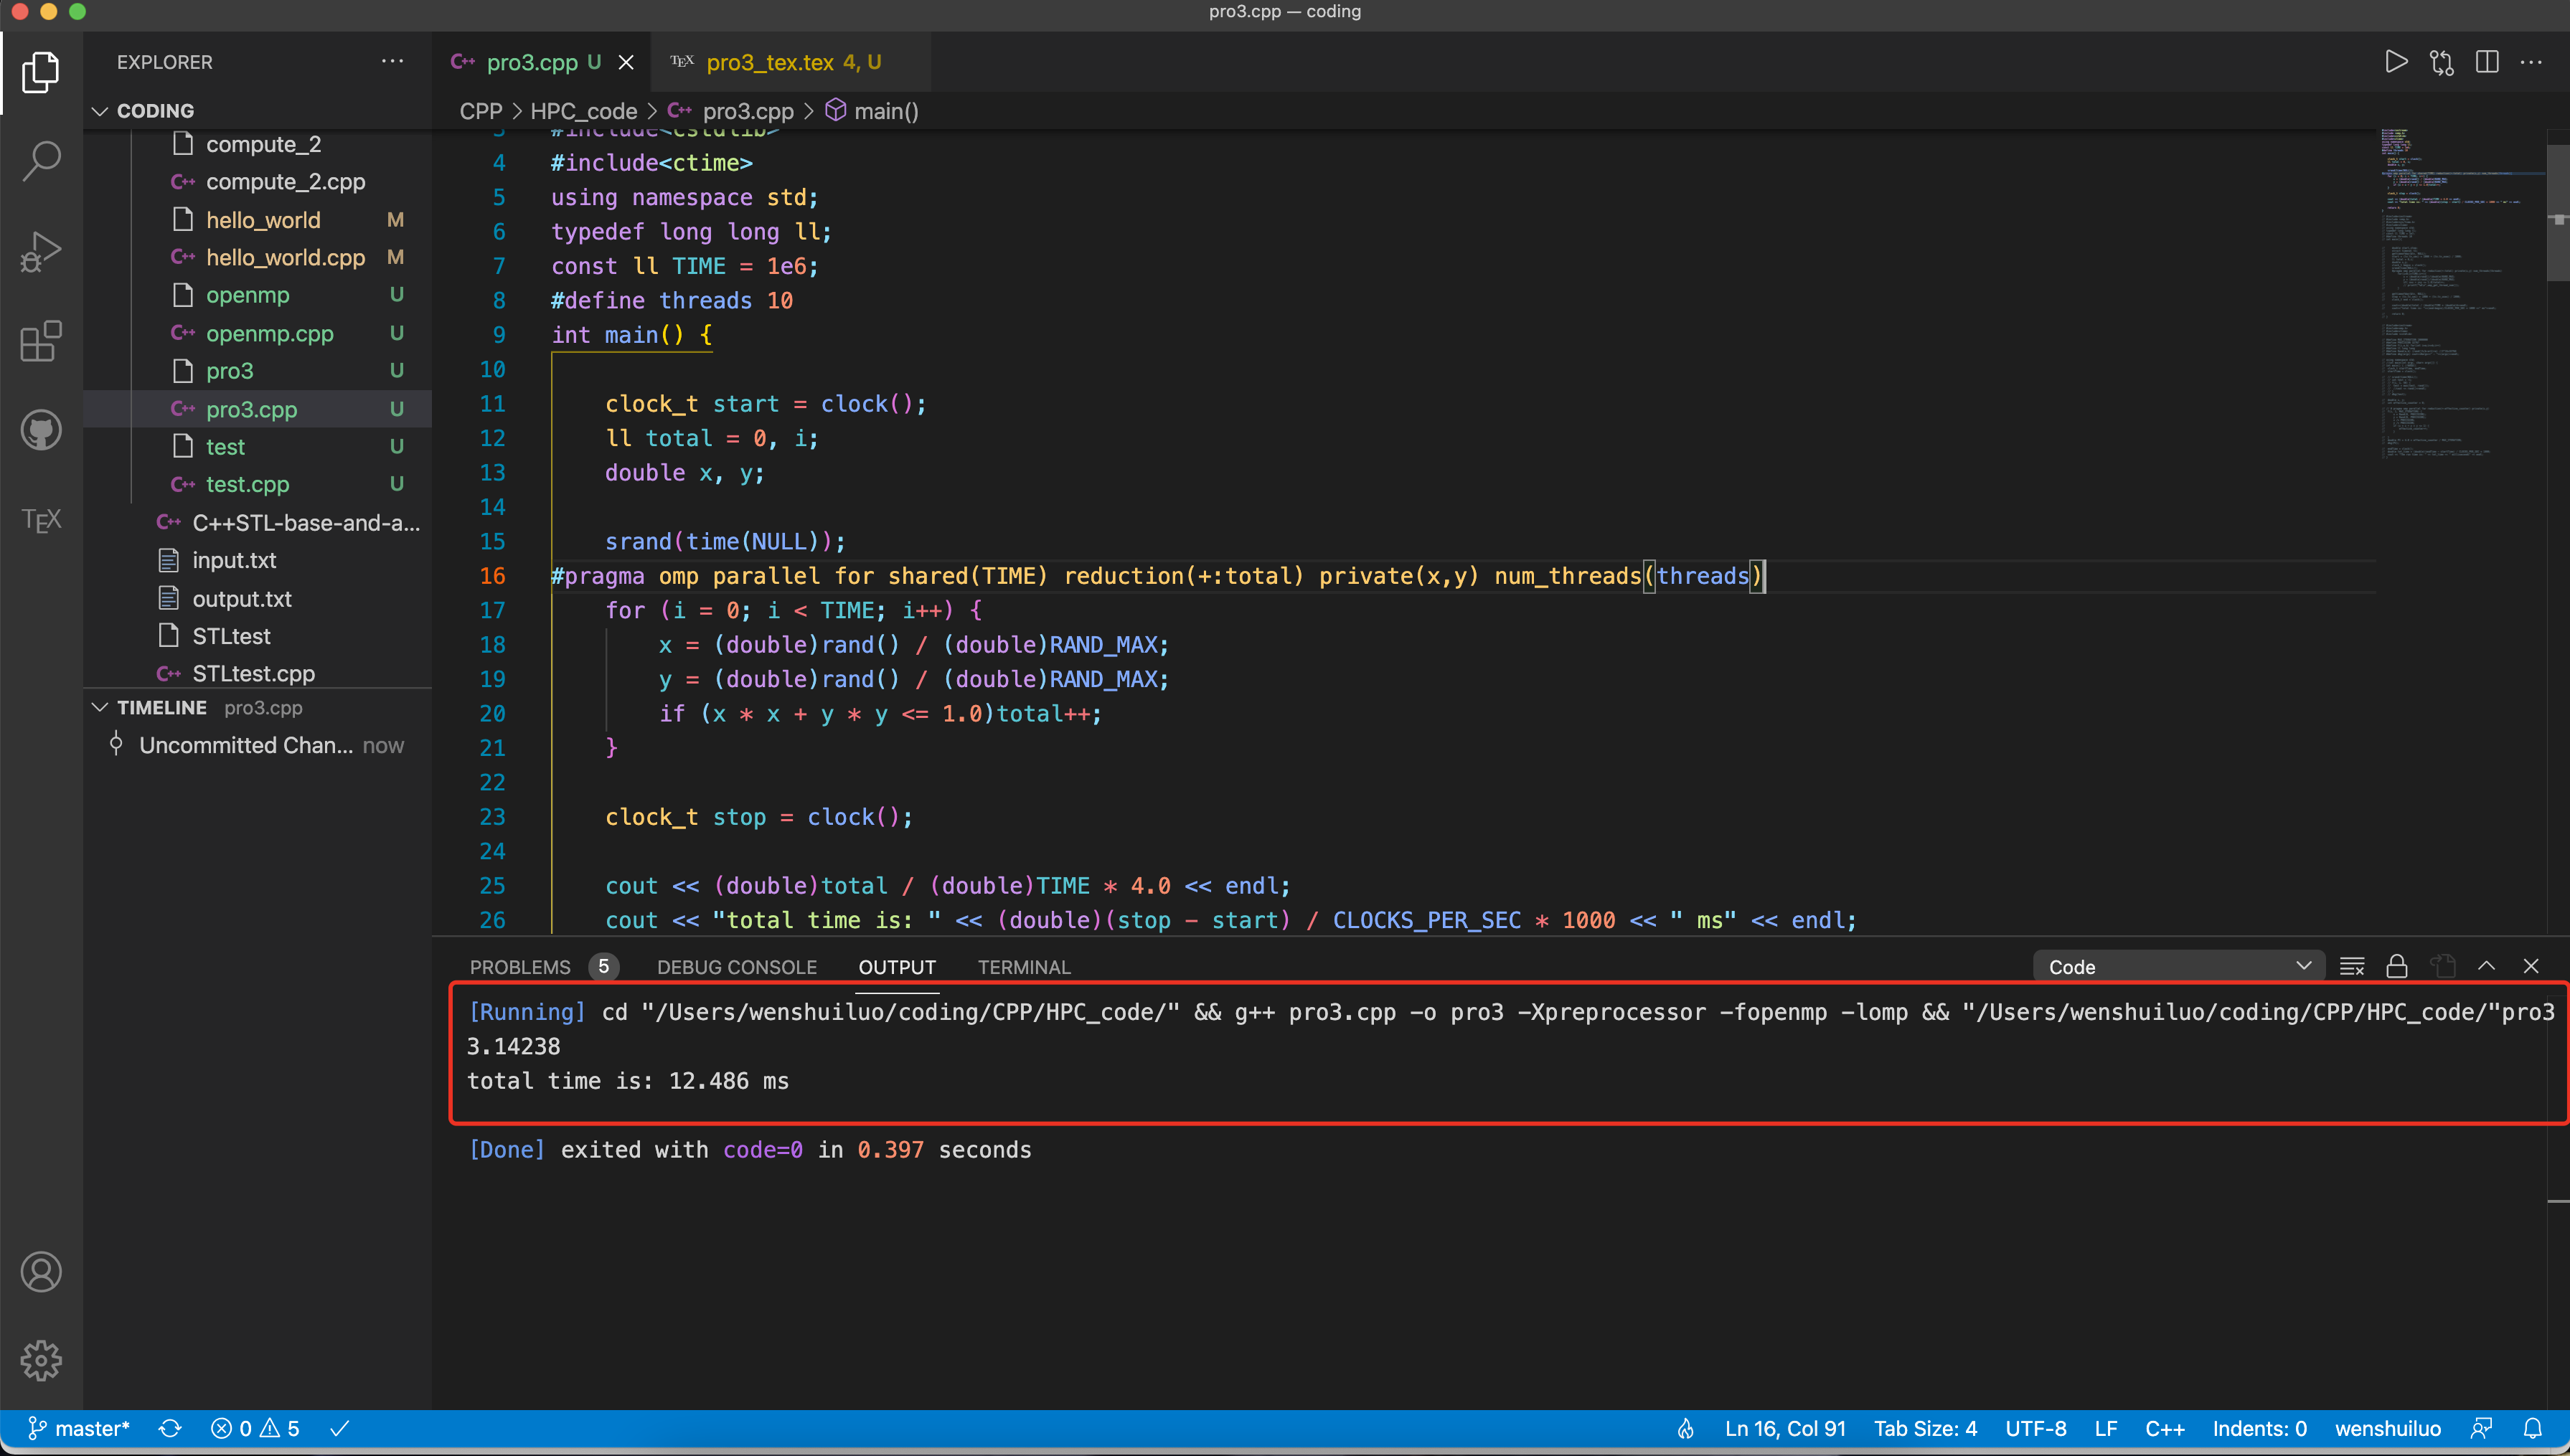
\includegraphics[width=1.0\textwidth]{omp2.png}
		\caption{openmp并行计算$\pi$值运行结果}
	\end{figure}

	未经过openmp并行加速的计算程序运行结果如图2所示,
	\begin{figure}[h]
		\centering
		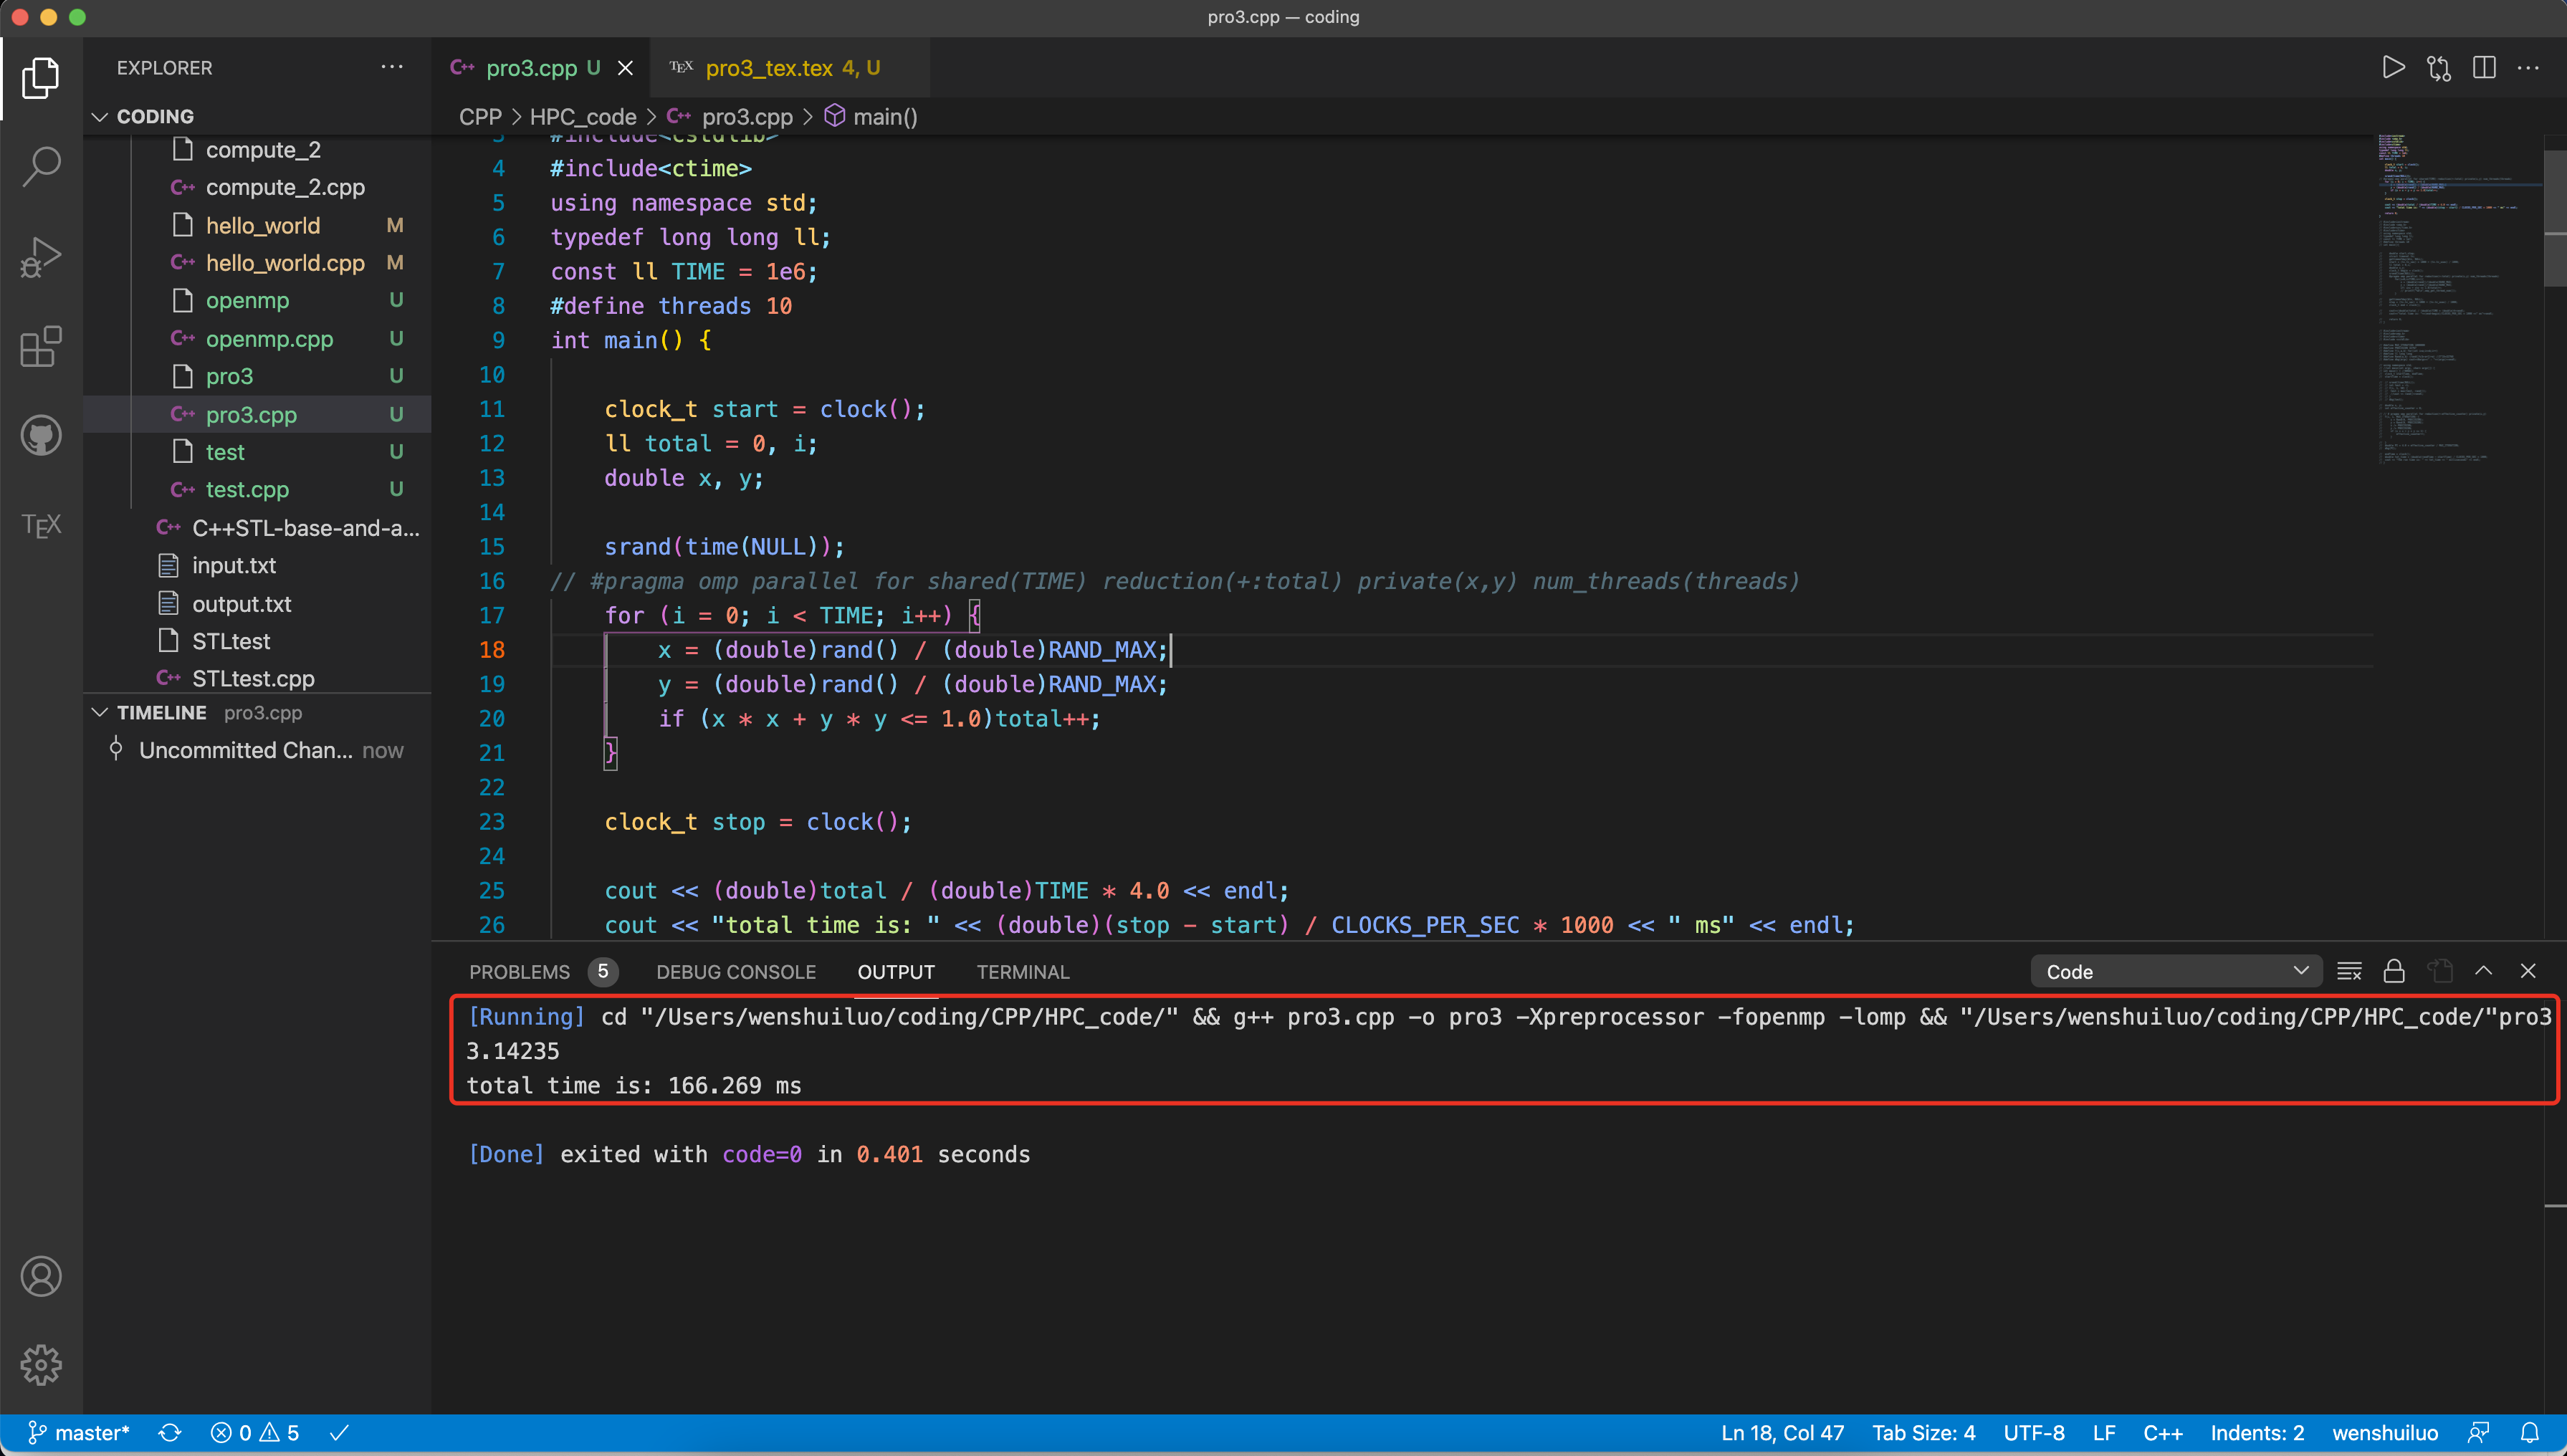
\includegraphics[width=1.0\textwidth]{omp1.png}
		\caption{未经过openmp并行计算的运行结果}
	\end{figure}
\end{document}
